\documentclass[10pt, a4paper]{article}

%%%%%%%%%%%%%%
%  Packages  %
%%%%%%%%%%%%%%


\usepackage{page_format}
\usepackage{special}
\usepackage{hyperref}
\usepackage{tikz}
\usepackage{pgfplots}
\usepackage[compat=1.1.0]{tikz-feynman}
\usepackage[font=small,labelfont=bf,
   justification=justified,
   format=plain]{caption}
\input{math_func}

\usepackage{slashed}

% References
\usepackage{biblatex}
\addbibresource{ref.bib}
\usetikzlibrary{intersections}

%%%%%%%%%%%%
%  Colors  %
%%%%%%%%%%%%
% ! EDIT HERE !
\colorlet{chaptercolor}{red!70!black} % Foreground color.
\colorlet{chaptercolorback}{red!10!white} % Background color

%%%%%%%%%%%%%%
% Page titre %
%%%%%%%%%%%%%%%
\title{Homework 3: Interstellar's Ring} % Title of the assignement.
\author{\PA} % Your name(s).
\teacher{Ruth Gregory} % Your teacher's name.
\class{Gravitational Physics} % The class title.

\university{Perimeter Institute for Theoretical Physics} % University
\faculty{Perimeter Scholars International} % Faculty 
%\departement{<Departement>} % Departement
\date{\today} % Date.


%%%%%%%%%%%%%%%%%%%%%%
% Begin the document %
%%%%%%%%%%%%%%%%%%%%%%
\begin{document}

% Make the title page.
\maketitlepage

% Make table of contents
\maketableofcontents

% Assignment starts here ----------------------------

\footnotesize{

\section{Setup}
We are interested in describing a Schwarzchild black hole of mass $M$ described by the Schwarzchild coordinates $(t', r', \theta', \phi')$. In this coordinate system, the singularity of the black hole is approached as $r' \to 0$ and the event horizon is the null hypersurface with $r' = 2GM$. The rotational symmetry of the system is broken by adding an accretion disk of external radius $a$ orbiting in the $\theta = \pi/2$ equatorial plane of the Schwarzchild coordinates. We are interested in the image of the light created by the accretion disk as seen by an observer at $r'\to \infty$. This observer will carry a local Minkowski coordinate system $(t, x, y, z)$. We take $t = t'$ forcing the observer to be static with respect to the black hole (using an infinitesimal acceleration to cancel its geodesic flow towards the black hole). The remaining coordinates $x, y, z$ are related to the asymptotic Schwarzchild coordinates $x', y', z'$ (respectively given by $r' \sin \theta' \cos \phi', r' \sin \theta' \sin \phi', \text{ and } r'\cos \theta'$) by a rotation. This rotation is fixed by taking $x = x'$ as the rotation axis and orienting the $z$ axis in the direction of the observer (note that this implies that the radius coordinate value $r = \sqrt{x^2 + y^2 + z^2} = r'$ is shared between the two systems, but refer to very different metrics at small $r$). The angle between $z$ and $z'$ is denoted $\theta_0$. 

The image at $r\to \infty$ is generated by the collection of light geodesic crossing the $xy$ plane parallel to the $z$ axis. For a given crossing point on the $xy$-plane we can time reverse (parameter reverse is more appropriate since the geodesic is null) the geodesic motion to see if this point is associated with an accretion disk initial condition and light the crossing point accordingly. The location of the crossing point on the $xy$ plane is identified with an angle $\phi = \text{arctan}_2(y, x)$ and a radius $b$ (the impact parameter of the geodesic at $r\to \infty$). An important feature of Schwarzchild geodesics is that they are planar: if the geodesic starts at an angle $\phi'$ on the accretion disk it will stay at the same angle. For a given impact parameter $b$ at angle $\phi$, there is a point of maximal approach to the black hole (periastron) with radius $r = r_0(b, \phi)$.  


\section{Warm up}
To better study geodesics around a Schwarzchild black hole, we use a different set of Schwarzchild coordinates $(t, r, \chi, \psi)$ (with the same time coordinate as the initial coordinate system) to simplify the calculations in the plane of motion. More precisely the plane of motion constitutes the equatorial plane $\chi = \pi/2$ of the coordinate system. Projecting all points of the geodesic on a constant $t$ slice, expressed in the polar coordinates $r, \psi$
of the equatorial plane. Finally, the $\psi = 0$ direction is aligned with the rays reaching the observer. 

\begin{enumerate}
  \item[(a)] Figure \ref{fig1} shows sketches of three geodesics in an equatorial plane orthogonal to the accretion disk. The red geodesic has impact parameter $b$ such that the point of the accretion disc plane reached by moving backward in parameter is out of the accretion disc. Geodesics $1$ and $2$ correspond to light reaching the observer. They have different periastra $r_0^1$ and $r_0^2$ and different impact parameters.
  \begin{figure}[h!]
    \centering
    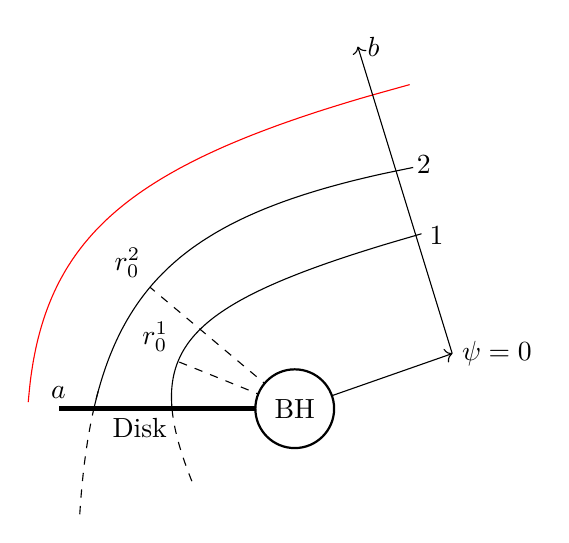
\begin{tikzpicture}[scale=2, rotate=0]
    
      % Define hyperbola parameters
      \def\a{1.2}
      \def\b{0.8}
      \def\c{-1}
    
      % Draw the hyperbola
      \draw[rotate=-22, dashed] plot[smooth,domain=-40:-19] ({\a*sec(\x)-2},{\b*tan(\x)});
      \draw[rotate=-40, dashed] plot[smooth,domain=-40:-22] ({1.5*\a*sec(\x-1) + \c -2},{2*\b*tan(\x-1)});
      \draw[rotate=-22] plot[smooth,domain=-19.5:59] ({\a*sec(\x)-2},{\b*tan(\x)});
      \draw[rotate=-40] plot[smooth,domain=-26:47] ({1.5*\a*sec(\x-1) + \c -2},{2*\b*tan(\x-1)});
      \draw[ultra thick] (0, 0) -- (-1.5, 0);
      \draw[rotate=-22, dashed] (0, 0) -- (-0.8, 0) node[above left] {$r_0^1$};
      \draw[rotate=-40, dashed] (0, 0) -- (-1.5 * 0.8, 0) node[above left] {$r_0^2$};

      \draw[rotate=-33, red] plot[smooth,domain=-28:54] ({1.5*\a*sec(\x-1) + \c -2.5},{2*\b*tan(\x-1)});

      \draw[->] (0, 0) -- (1, 0.35) node[right] {$\psi = 0$};
      \draw[fill=white, thick] (0,0) circle [radius=0.25];

      \draw (0.9,1.1) node {$1$};
      \draw (0.82,1+0.55) node {$2$};
      \draw (-1.5,0) node[above ] {$a$};
      \draw (-1.5/2,0) node[below left] {Disk};

      \draw[->] (1, 0.35) -- (3*0.8-3+1, 3-3*0.35+0.35) node[right] {$b$};
      
      \draw (0,0) node {BH};
    \end{tikzpicture}
    \caption{Equatorial plane sketch of geodesic motion with three different impact parameters and periastra \label{fig1}. The periastra gets further away from the accretion disk point as we get closer to the outer ring of the accretion disk. If the disk was large, the geodesic starting on the outer ring would approximatively be a straight line starting at the disk point and directed towards the observer. In this limit, the periastron is located exactly in the middle of the line. In this sketch the example geodesic are curving in the clockwise direction relative to the $\psi = 0$ axis. This is why Figures \ref{fig2} and \ref{fig3} are plotted against $-\psi$ (making the deflexion angles negative)}
  \end{figure}
\newpage
  \item[(b)] Figure \ref{fig2} compares the total deflexion angle for the two geodesics presented in \ref{fig1}.
  \begin{figure}[h!]
    \centering
    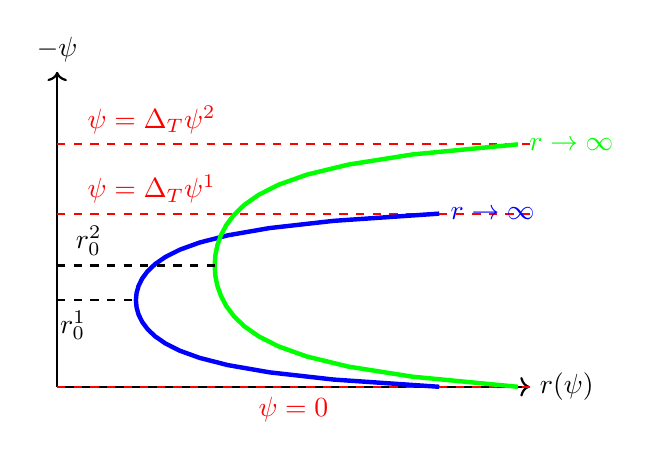
\begin{tikzpicture}[domain=-4:7] [scale=2]
      \draw[thick, ->] (0,0) -- (6,0) node[right] {$r(\psi)$};
      \draw[thick,->] (0,0) -- (0,4) node[above] {$-\psi$};
      \draw[thick, red, dashed] (0,.35*pi*2) -- (6,.35*pi*2) node[pos=0.2, above] {$\psi = \Delta_T \psi^1$};
      \draw[thick, red, dashed] (0,.35*pi*2*1.4) -- (6,.35*pi*2*1.4) node[pos=0.2, above] {$\psi = \Delta_T \psi^2$};
      \draw[thick, red, dashed] (0,0) -- (6,0) node[midway, below] {$\psi = 0$};
      \draw[ultra thick,color=blue] plot[domain=-.35*pi:.35*pi] ({1+tan(\x r)*tan(\x r)}, \x+0.35*pi) node[right] {$r\to \infty$};
      \draw[ultra thick,color=green] plot[domain=-.35*pi:.35*pi] ({2+tan(\x r)*tan(\x r)}, 1.4*\x+1.4*0.35*pi) node[right] {$r\to \infty$};
      \draw[thick, dashed] (0, 0.35*pi) -- (1, 0.35*pi) node[pos=0.2, below] {$r_0^1$};
      \draw[thick, dashed] (0, 1.4*0.35*pi) -- (2, 1.4*0.35*pi) node[pos=0.2, above] {$r_0^2$};
    \end{tikzpicture}
    \caption{$\psi$ coordinate describing geodesics $1$ (blue) and $2$ (green) from \ref{fig1} as a function of the respective radial coordinate $r$. The full geodesics (extended beyond the accretion disc) start at $r \to \infty$ and end again at $r\to \infty$. We choose $\psi = 0$ to represent the observer angle for both geodesic forcing them to coincide on the $\psi = 0$ axis. The other asymptote represents the extended initial direction of motion of light consistent with the initial accretion disc point. The minimal value of $r$ (the periastron) is realized in the middle of the geodesic motion. From the dashed lines in \ref{fig1}, we see that the total deflexion angle $\Delta_T \psi^{1, 2}$ between $\phi = 0$ and the extended motion asymptote is smaller for geodesic $1$ compared to geodesic $2$ (we have $\Delta_T \psi^{1} < \Delta_T \psi^{2}$). This is consistent with the increasing gravitational pull with decreasing pariastron. \label{fig2}}
  \end{figure}
  \item[(c)] Figure \ref{fig3} represents the same goedesics as figure \ref{fig2}, but has the radial coordinate $r$ replaced by the inverse radial coordinate $u = 1/r$.
  \begin{figure}[h!]
    \centering
    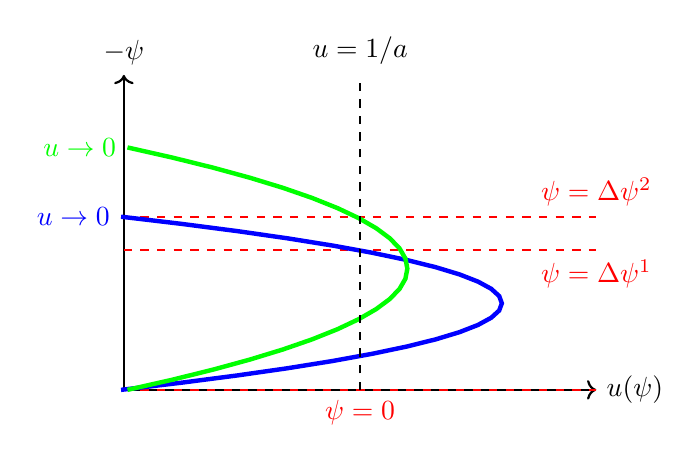
\begin{tikzpicture}[domain=-4:7] [scale=2]
      \draw[thick, ->] (0,0) -- (6,0) node[right] {$u(\psi)$};
      \draw[thick,->] (0,0) -- (0,4) node[above] {$-\psi$};
      \draw[thick, red, dashed] (0,.35*pi*2) -- (6,.35*pi*2) node[pos=1, above] {$\psi = \Delta \psi^2$};
      \draw[thick, red, dashed] (0,.35*pi*2*1.4-1.3) -- (6,.35*pi*2*1.4-1.3) node[pos=1, below] {$\psi = \Delta \psi^1$};
      \draw[thick, red, dashed] (0,0) -- (6,0) node[midway, below] {$\psi = 0$};
      \draw[ultra thick,color=blue] plot[domain=-.35*pi:.35*pi] ({4*(0.2+1-\x*\x)}, \x+0.35*pi) node[left] {$u\to 0$};
      \draw[ultra thick,color=green] plot[domain=-.35*pi:.35*pi] ({1.5*(0.4+2-1.4*1.4*\x*\x)}, 1.4*\x+1.4*0.35*pi) node[left] {$u\to 0$};
      %\draw[thick, dashed] (0, 0.35*pi) -- (3*0.2+3, 0.35*pi) node[pos=0, left] {$u_0^1 = 1/r_0^1$};
      %\draw[thick, dashed] (0, 1.4*0.35*pi) -- (2.5*0.4+5, 1.4*0.35*pi) node[pos=0, left] {$u_0^2 = 1/r_0^2$};
      \draw[thick, dashed] (3, 0) -- (3, 4) node[pos=1, above] {$u = 1/a$};
    \end{tikzpicture}
    \caption{$\psi$ coordinate describing geodesics $1$ (blue) and $2$ (green) from \ref{fig1} as a function of the respective inverse radial coordinate $u = 1/r$. We define the partial deflexion angle $\Delta \psi^{1, 2}$ as the angle between the observer direction ($\psi = 0$) and the first crossing of the $u=1/a$ surface by the geodesic (accretion disk point). Since there are two crossing points, we have to specify which one corresponds to the disk. \label{fig3}}
  \end{figure}\\
  Note: The convention used in the previous figures is different from the one used in the assignement. The assignment convention uses the extended motion initial asymptote as the $\psi=0$ direction. This implies that the total deflexion angle consistent with this convention is $-\Delta_T \psi^{1, 2}$ since it is measured between the same asymptotes, but with reversed order. The partial deflexion angle consistent with the assignment convention is $-(\Delta_T\psi^{1, 2}-\Delta\psi^{1, 2})$ where the global sign takes the relative orientations into account.
\end{enumerate}
% does this happen with stars ?
\newpage
\section{Null geodesics in a Schwarzchild's spacetime}

\section{The observer's frame}

\section{Drawing the observed disk}

\section{Acknowledgement}

Chat GPT was used to produce the initial code for the figures in the Warm up section.

}

% References
\makereferences
%-------------------------------------------------------


%%%%%%%%%%%%%%%%%%%%%%%%
% Terminer le document %
%%%%%%%%%%%%%%%%%%%%%%%%
\end{document}
